%%!TEX root = ../main.tex
%
%
%\section{Results}

To quantify the end-to-end learned navigation, the primary metric is success rate. This is simply a measure of the vehicle's ability to reach the destination without colliding with any obstacles. For this metric, any collision, regardless of severity, is considered a failure and the simulation is terminated. In addition to the primary metric, the length of the path is analyzed relative to the PSO path. Since the PSO path would generally be able to find a shorter path than the trained algorithm, which only has local information, the comparison will be used to show that the path taken by the trained algorithm is reasonable, and not simply a path that avoids obstacles yet produces bizarre trajectories.

When testing the effect of hilliness on navigation, the maximum height of the random height map was increased from 0 m (flat) to 12 m in increments of 2 m. At each level, 200 simulations on random height maps generated using simplex noise were performed to understand the success rate of the algorithm with respect to the terrain change. The results are shown in Fig. \ref{fig:rigid_height_success}. As expected, the trained network's ability to safely navigate the environment decreases with increased hilliness. Additionally, as the number of obstacles is increased, the task becomes more difficult. Tests conducted with 20 obstacles represent the closest point to the training environment.

In addition to the increasing height tests, experiments were conducted with hilliness of 0 m and 6 m with three terrain models: undeformable (rigid), hard-deformable, and soft-deformable. Since no deformable terrain was experienced in training, this is also a measure of policy robustness with respect to the terrain. These results, for varying terrain, heights, and obstacles are shown in Fig. \ref{fig:obstacles_hilly_and_flat_success}. While the policy can maintain relatively high success on deformable soil when the terrain is flat, the combination of deformable and hilly terrain proves difficult for the policy with success rates falling below 50\%.

\begin{figure}
    \captionsetup{justification=centering}
    \centering
    \begin{subfigure}{0.36\textwidth}
        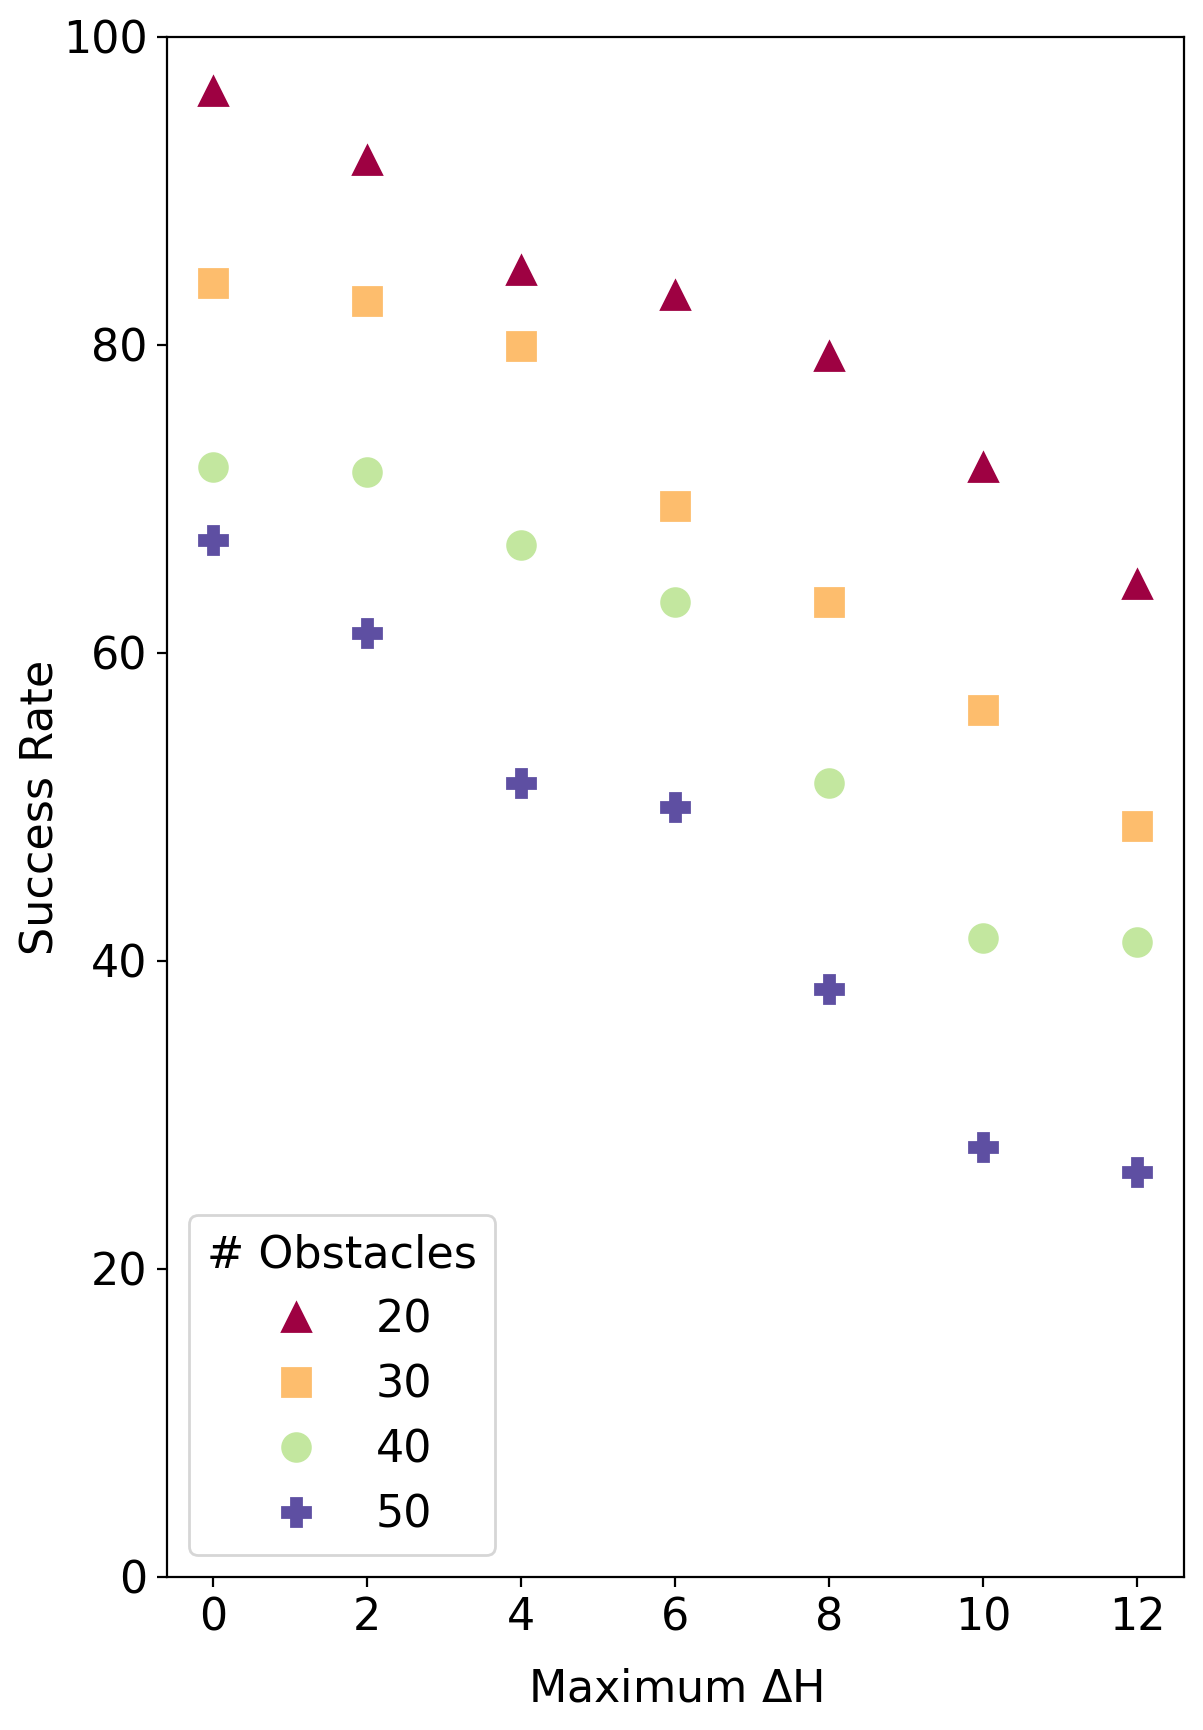
\includegraphics[height=.25\paperheight]{images/demonstration/rigid_height_success_rate.png}
        \caption{Success rate in \% vs hilliness on rigid terrain.}
        \label{fig:rigid_height_success}
    \end{subfigure}%
    \hfill
    \begin{subfigure}{0.44\textwidth}
        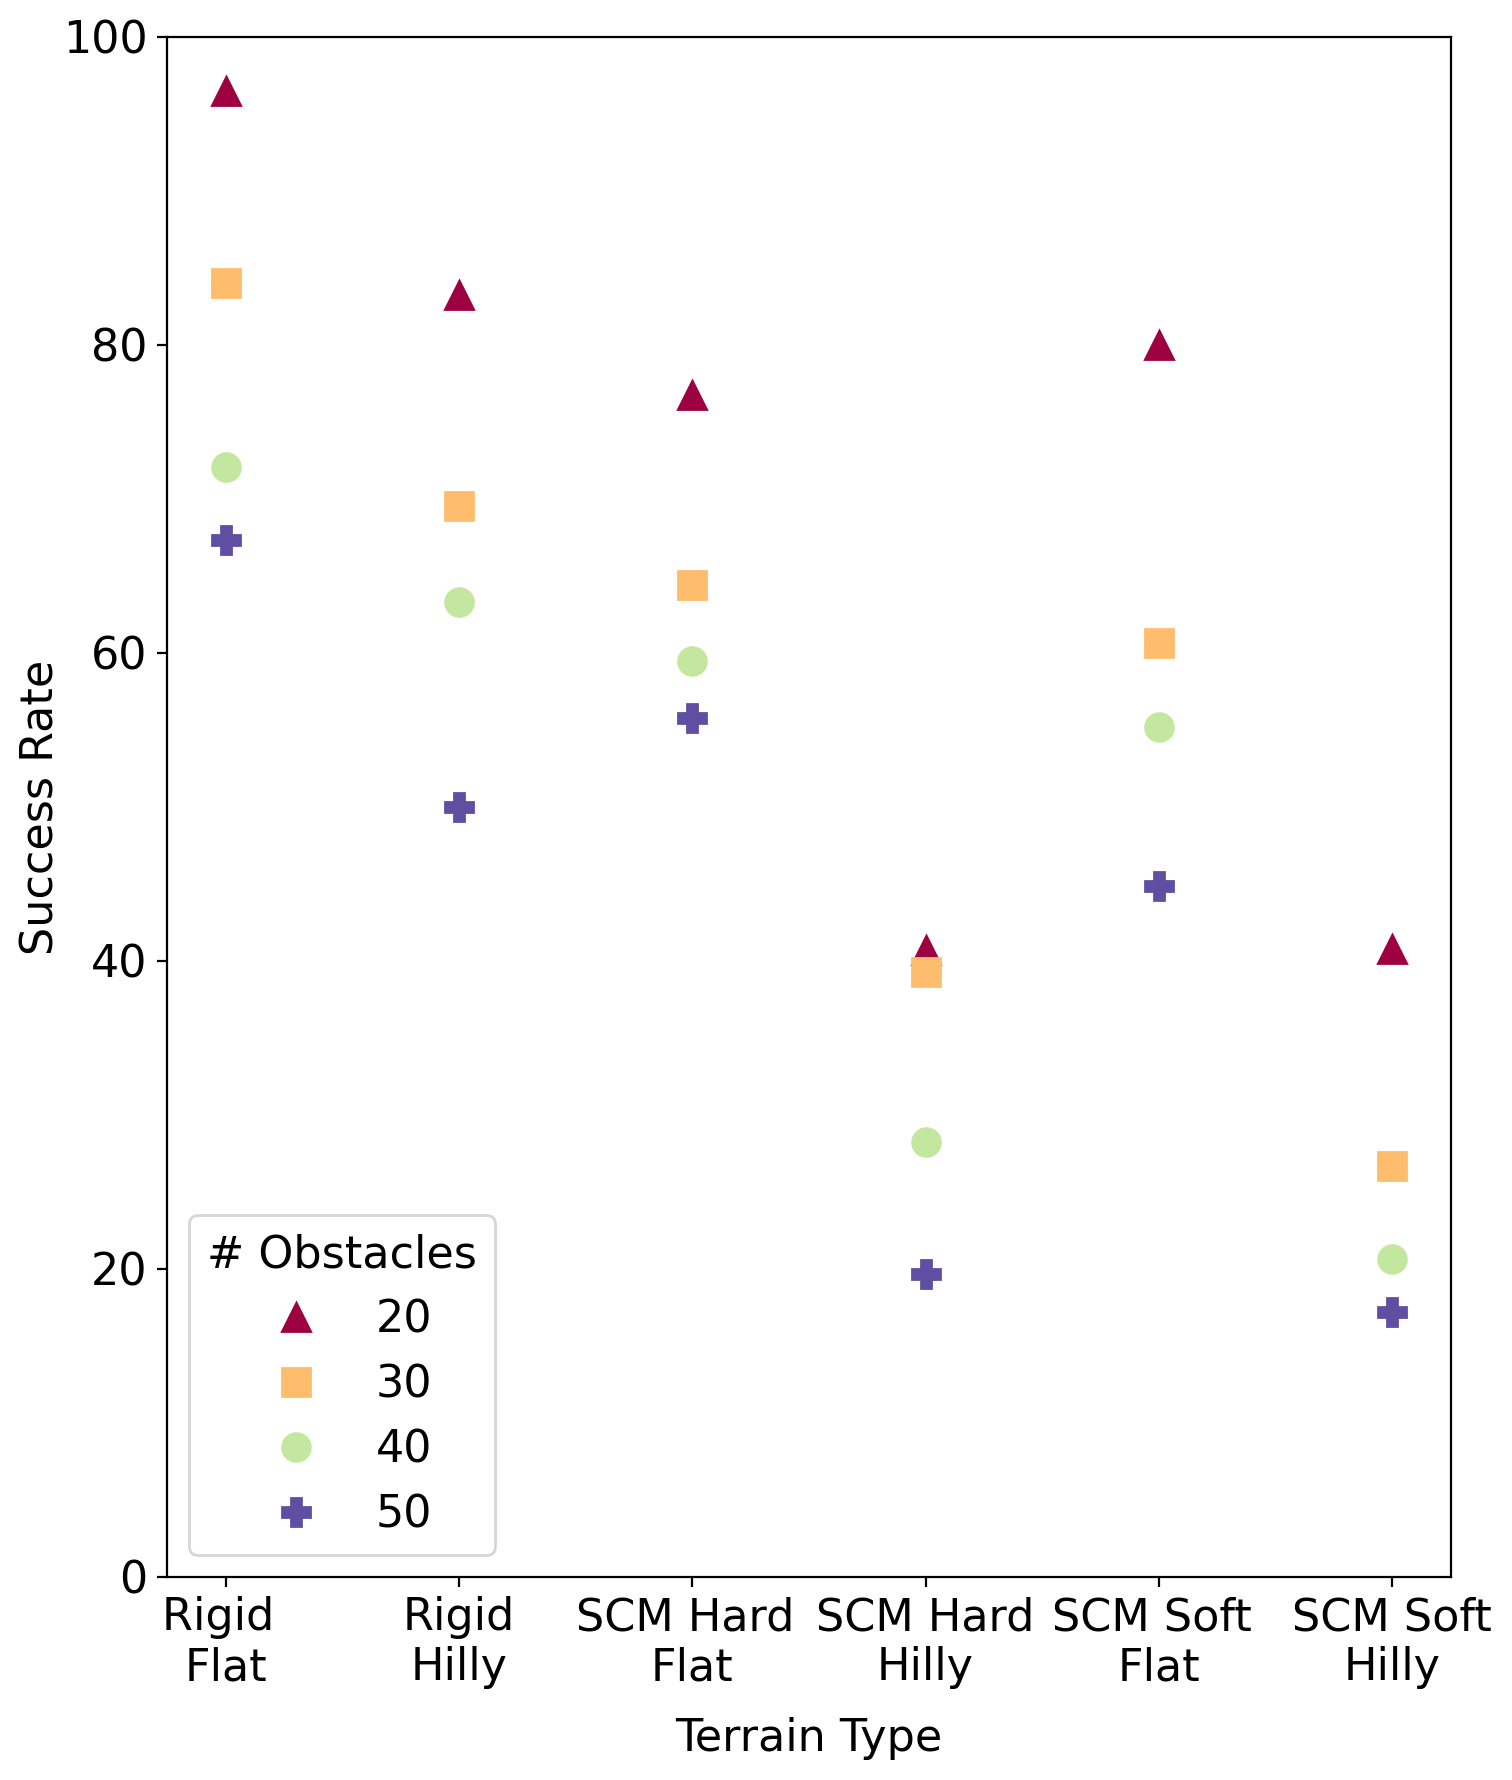
\includegraphics[height=.25\paperheight]{images/demonstration/terrain_obstacles_flat_and_height_success_rate.png}
        \caption{Success rate in \% vs hilly and flat terrains with varying stiffness.}
        \label{fig:obstacles_hilly_and_flat_success}
    \end{subfigure}
    \caption{Success rate when increasing complexity of the terrain.}
    \label{fig:successRates}
\end{figure}

The second metric, which compares the length of the chosen path to the length of a path generated by the PSO, is discussed for a single environment setup. This is shown in Fig. \ref{fig:pso_length_compare} for flat, rigid terrain with 50 obstacles, which is more than double the obstacle density used in training. The length difference is computed as $length(NN path) - length(PSO path)$. These results show that the mode of the distribution is around -5 m, meaning the NN path is most often 5 m longer than the PSO path. While a direct comparison is not feasible since the PSO takes into account global knowledge and does not make any claims about optimality, the path taken by the NN appears to be moderately close in length to a global planner. This means that the policy is appropriately weighting the directness of the path as expected. Only successful paths were included in the calculation of this metric.

To further understand and analyze the success rate of the algorithm, the full set of collisions were evaluated based on the directness of collision. The directness of collision was computed by measuring the overlap of the projection of the vehicle and obstacle onto a plane perpendicular to the vehicle heading. This metric quantifies scraping collisions near 0\% and direct collisions near 100\%. This percentage can be interpreted as the percent of the frontal area of the vehicle that collided with the obstacle. While this cannot directly assign severity to the collision, it can hint at the type of collisions experienced by the policy. The distribution of results in Fig. \ref{fig:rigid_failure_metric_histogram} show that while the mode is near 100\%, there is also a significant portion of the collisions that have low directness. %This suggests that further analysis and adjustments could be made to the training to understand if increased penalty to force the vehicle away from obstacles could improve the success rate further.

\begin{figure}
    \captionsetup{justification=centering}
    \centering
    \begin{subfigure}{0.45\textwidth}
        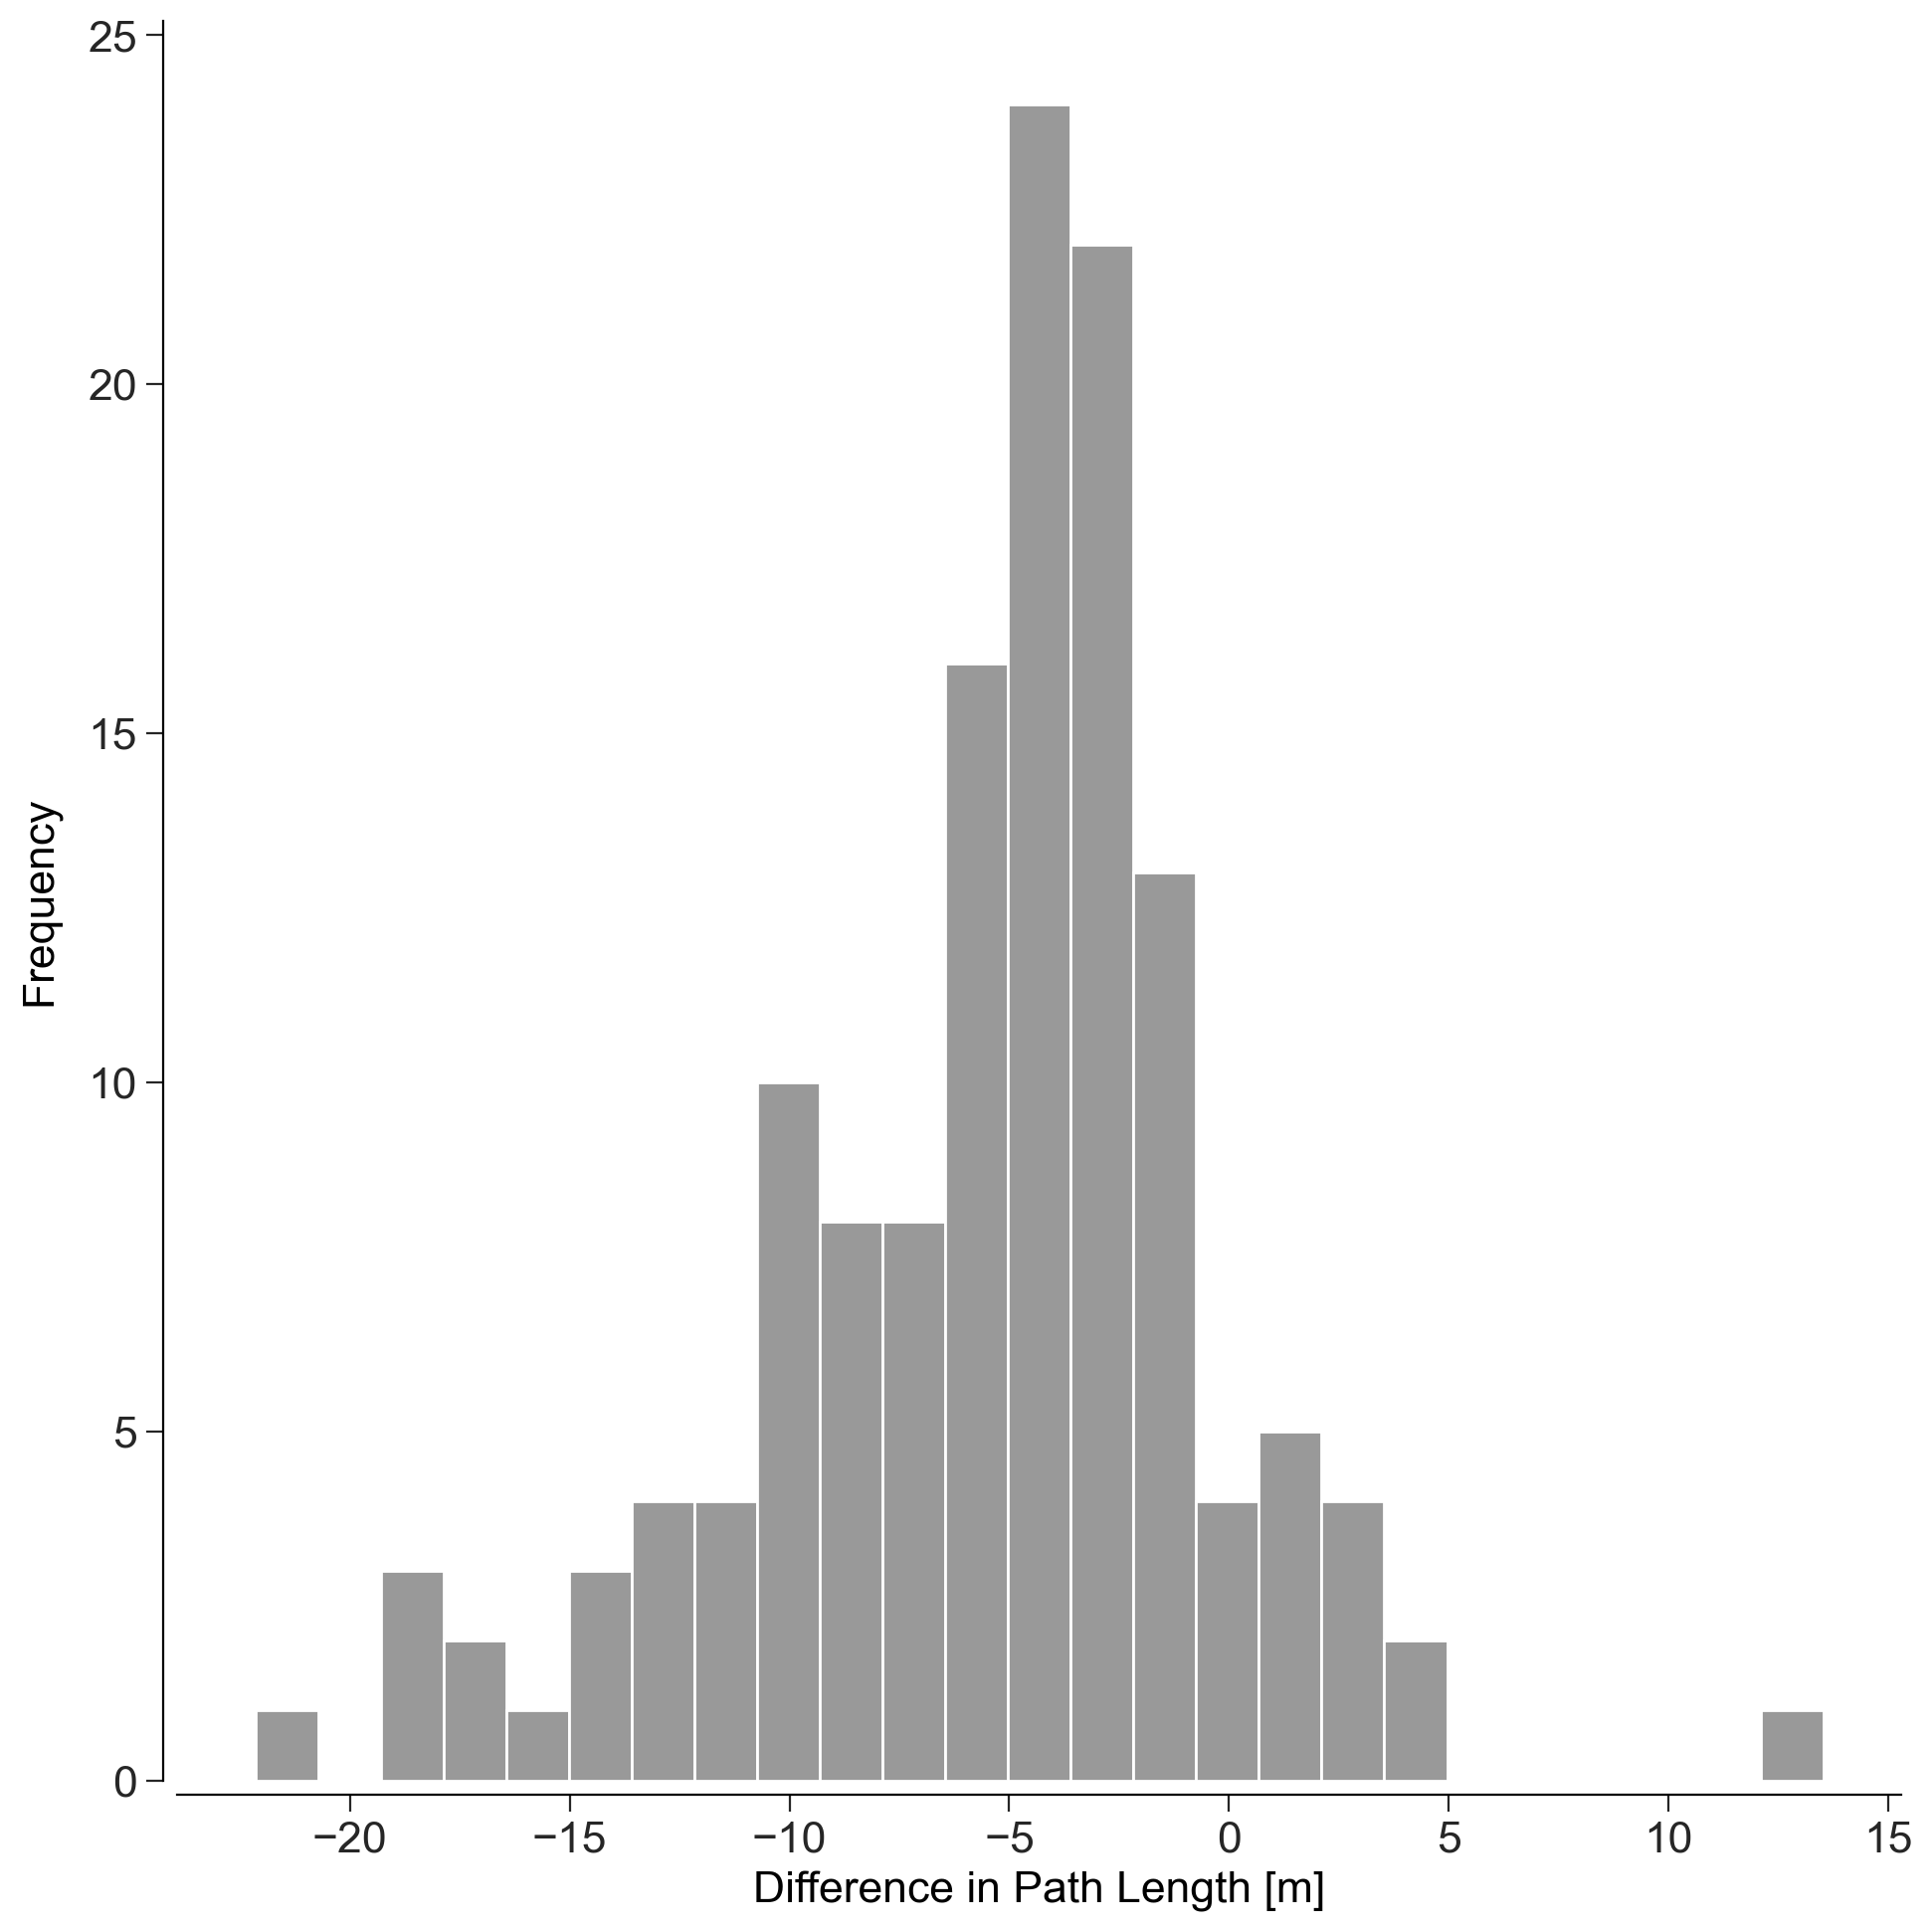
\includegraphics[height=.22\paperheight]{images/demonstration/rigid_9_pso_metric_histogram.png}
        \caption{Difference in path length between the pso trajectory and vehicle path for flat rigid terrain with 50 obstacles.}
        \label{fig:pso_length_compare}
    \end{subfigure}%
    \hfill
    \begin{subfigure}{0.45\textwidth}
        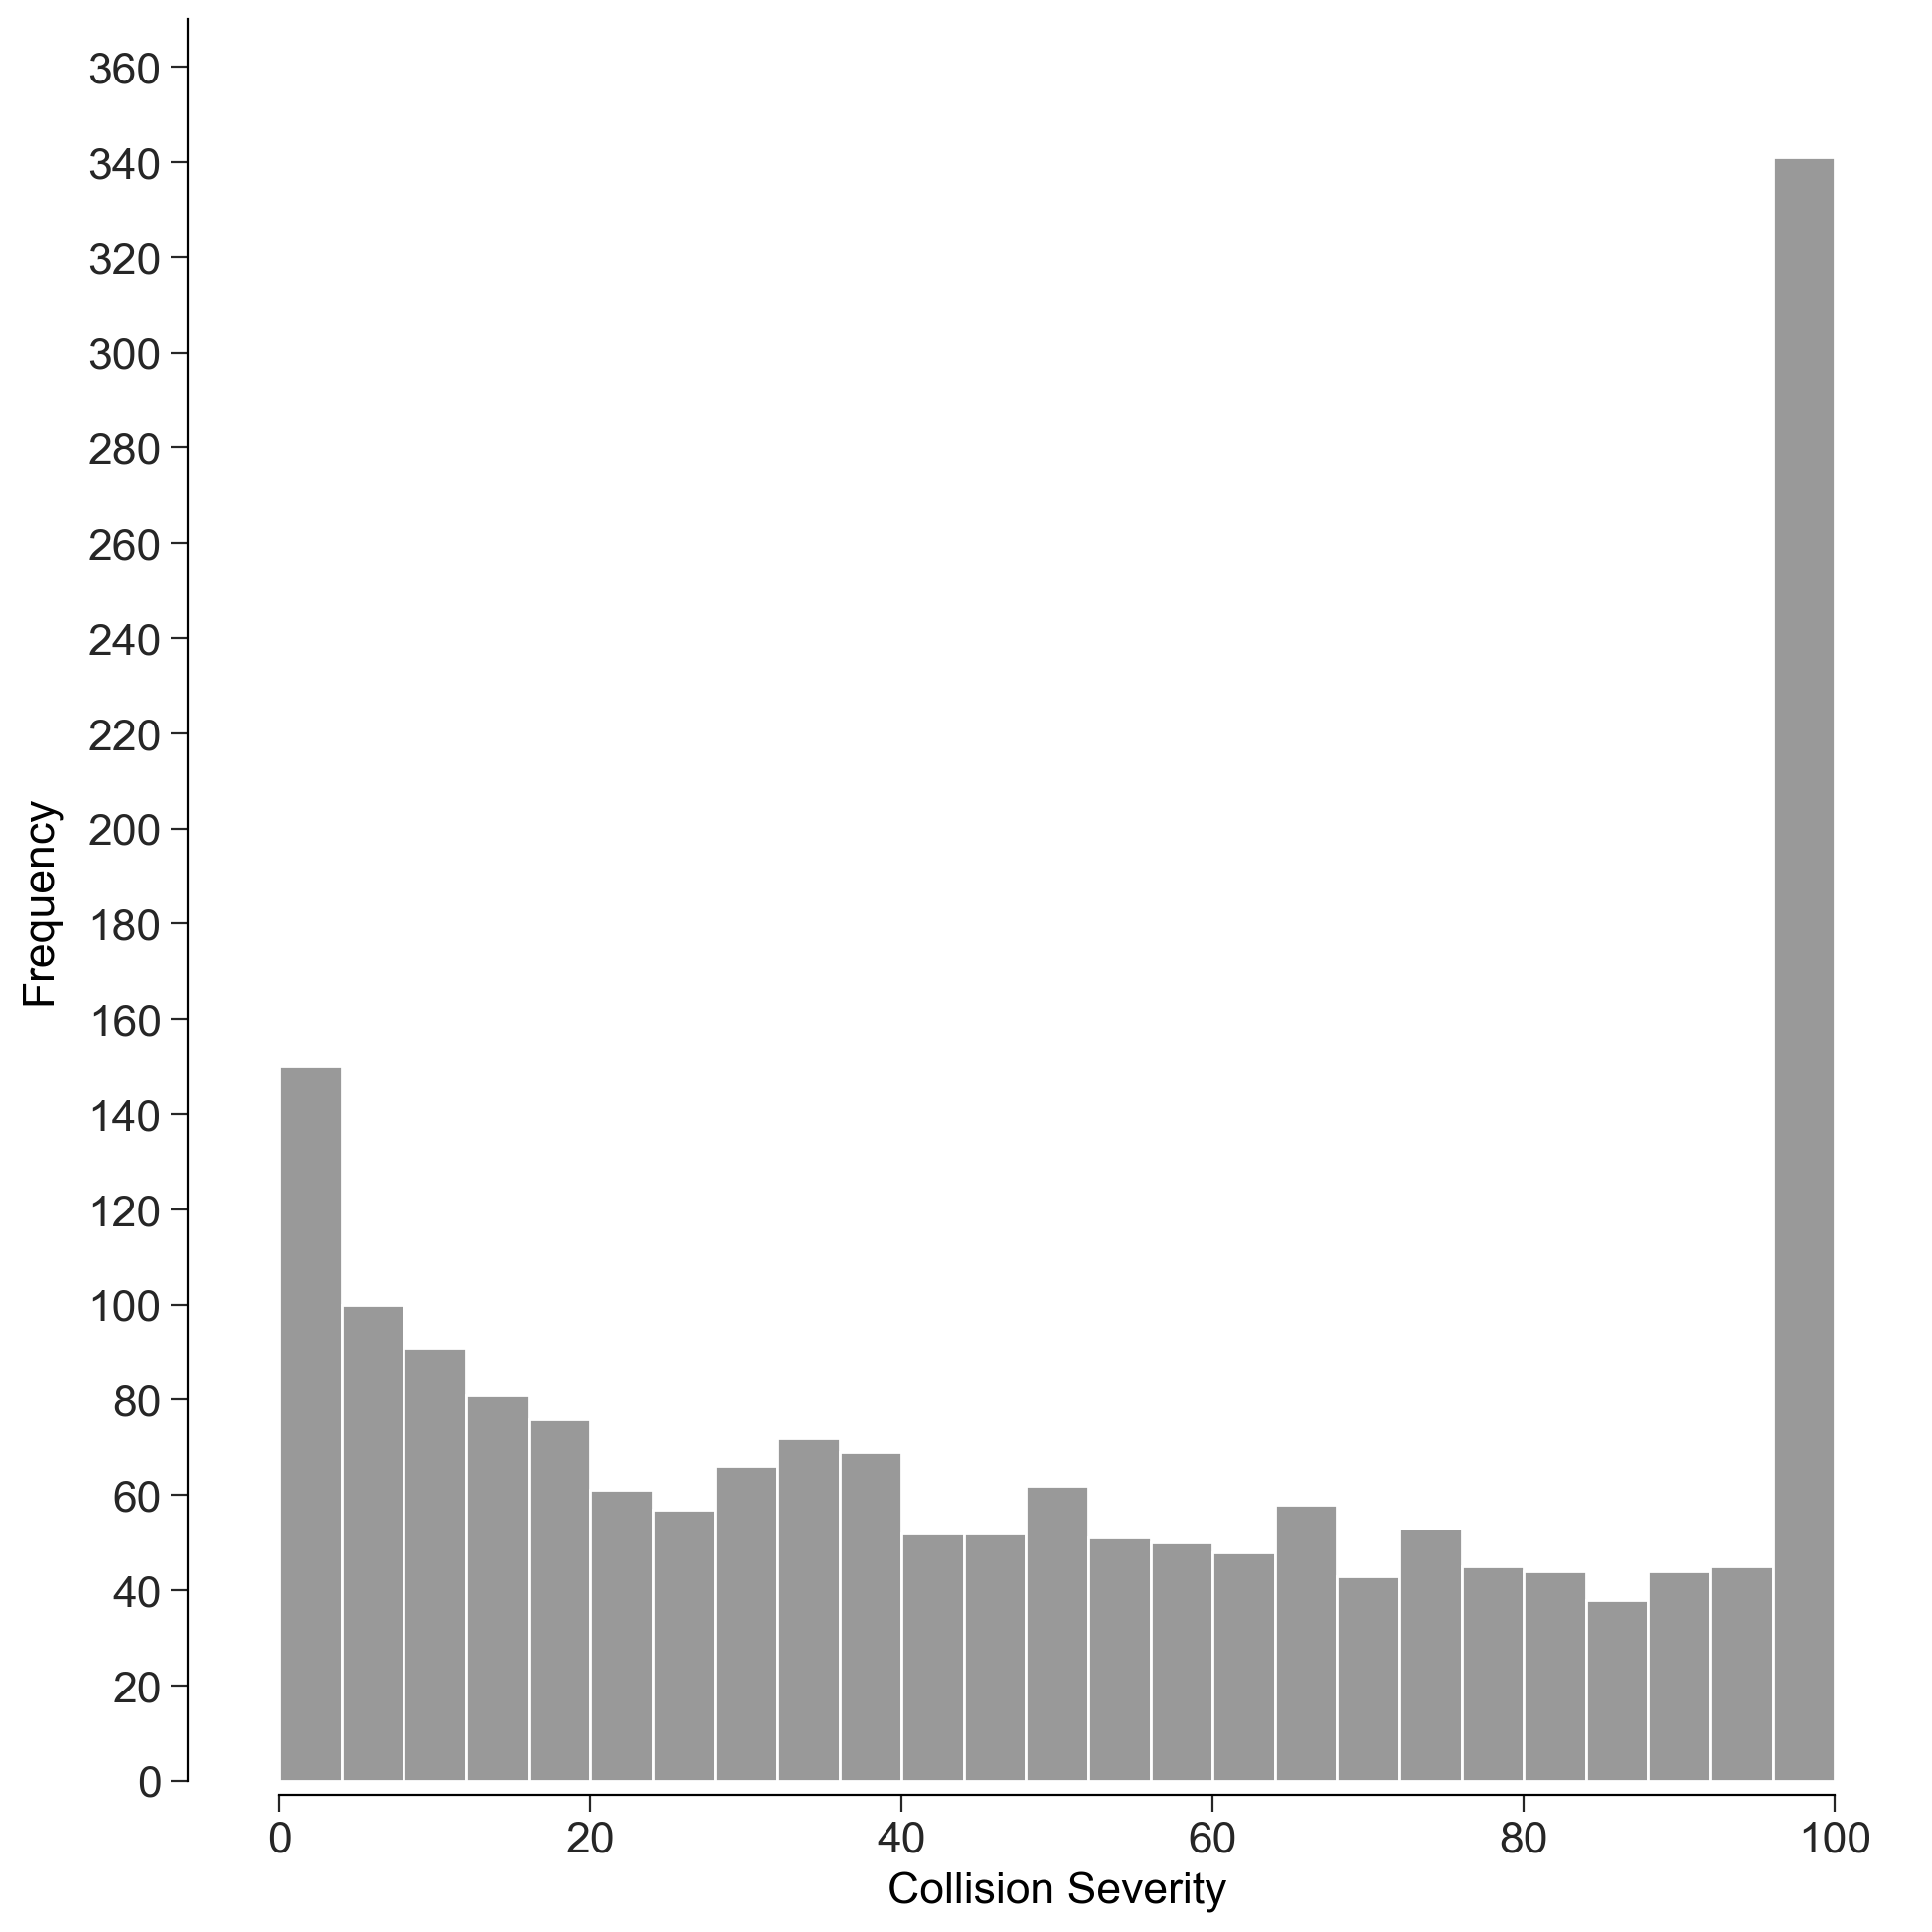
\includegraphics[height=.22\paperheight]{images/demonstration/rigid_failure_metric_histogram.png}
        \caption{Failure severity on flat rigid terrain for all obstacle configurations.}
        \label{fig:rigid_failure_metric_histogram}
    \end{subfigure}
    \caption{Additional metrics analyzing path length and collision directness.}
\end{figure}
